\documentclass[tikz]{standalone}
\usetikzlibrary{decorations.pathmorphing}

\begin{document}
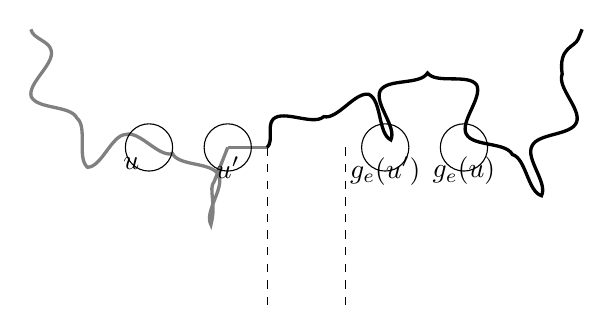
\begin{tikzpicture}
    % Define the coordinates
    \coordinate (u) at (0,0);
    \coordinate (u') at (1,0);
    \coordinate (geu') at (3,0);
    \coordinate (geu) at (4,0);

    % Draw the original walk in gray
    \draw[gray, very thick, decorate, decoration={snake, segment length=10mm, amplitude=2mm}] 
        (-1.5,1.5) .. controls (-1,-1) and (0.5,1) .. (u) 
        .. controls (0.5,-1) .. (u');
    \draw[gray, very thick] (u') -- (1.5,0);
    
    % Draw the modified walk in black
    \draw[very thick, decorate, decoration={snake, segment length=10mm, amplitude=2mm}] 
        (1.5,0) .. controls (2,0.5) .. (geu')
        .. controls (3.5,1) .. (geu)
        .. controls (4.5, -1) .. (5.5,1.5);
    
    % Draw circles around the points to emphasize reflection
    \foreach \point in {u, u', geu', geu} {
        \draw[thin] (\point) circle (0.3);
    }

    % Label the points
    \draw (u) node[below left] {$u$} 
          (u') node[below] {$u'$}
          (geu') node[below] {$g_e(u')$}
          (geu) node[below] {$g_e(u)$};

    % Draw lines for the reflection
    \draw[thin, dashed] (1.5,0) -- (1.5, -2);
    \draw[thin, dashed] (2.5,0) -- (2.5, -2);
\end{tikzpicture}
\end{document}